\subsection{Terrain modification}
Even though the problem with terrain generation was solved, as indicated in \autoref{subsec:spherical_problem_terrain_gen}, we didn't manage to find a remedy for a problem that has to do with terrain modification.
When the terrain modification is carried out on the boundary of one region, it has to be accompanied by a "secondary" modification in the second region.
Otherwise, visible gaps will emerge.
Our attempted solution was to calculate the center of secondary modification as
$$\frac{c - c_1}{\lVert c - c_1 \rVert}(R + (R - \lVert c - c_1 \rVert)) + c_2 = \frac{c - c_1}{\lVert c - c_1 \rVert}(2R - \lVert c - c_1 \rVert) + c_2,$$
where $c$ is the user-selected center of modification, $c_1$ and $c_2$ are centers of the first and second region, and $R$ is the radius of the region.

This, however, doesn't solve the problem, as the two modifications are mismatched, as can be seen in \autoref{fig:gaps-bt-regions-spherical}.
\begin{figure}[!htb]
    \centering
    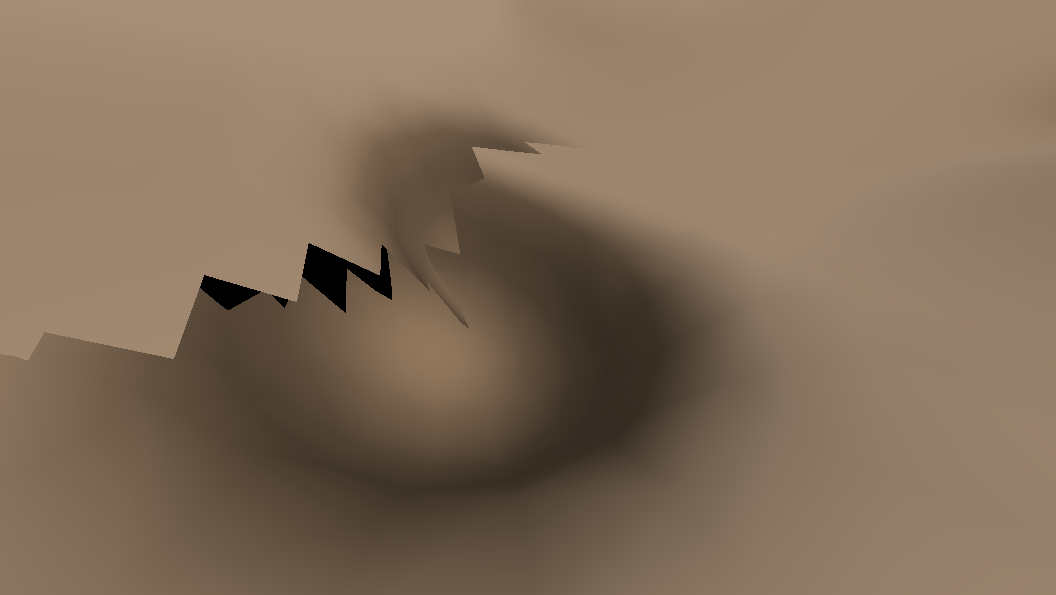
\includegraphics[width=0.6\textwidth]{chapters/problems/resources/gaps-bt-regions-mining.png}
    \caption{Gaps between regions in spherical space after terrain modification}
    \label{fig:gaps-bt-regions-spherical}
\end{figure}